% !TeX program = xelatex
\documentclass[UTF8,a4paper,10pt,twocolumn,fontset=none]{ctexart}

\usepackage{iftex}
\ifXeTeX\else
  \PackageError{event-alpha-paper}{This document must be compiled with XeLaTeX}
  {In Overleaf, open Menu -> Settings -> Compiler and select XeLaTeX.}
\fi

\setCJKmainfont{FandolSong-Regular}
\setCJKsansfont{FandolHei-Regular}
\setCJKmonofont{FandolFang-Regular}

\usepackage[left=1.55cm,right=1.55cm,top=1.55cm,bottom=1.6cm,columnsep=0.68cm]{geometry}
\usepackage{amsmath,amssymb,booktabs,tabularx,array,multirow}
\usepackage{graphicx,subcaption,float,enumitem,hyperref,xcolor,microtype}
\usepackage[section]{placeins}
\usepackage{tikz}
\usetikzlibrary{arrows.meta,positioning,shapes.geometric}

\hypersetup{
  colorlinks=true,
  linkcolor=black,
  citecolor=blue!55!black,
  urlcolor=blue!55!black
}

\setlength{\parindent}{2em}
\setlength{\parskip}{0pt}
\setlength{\columnsep}{0.68cm}
\setlength{\floatsep}{7pt plus 2pt minus 1pt}
\setlength{\textfloatsep}{8pt plus 2pt minus 2pt}
\setlength{\intextsep}{7pt plus 2pt minus 1pt}
\setlength{\abovecaptionskip}{3pt}
\setlength{\belowcaptionskip}{0pt}
\renewcommand{\topfraction}{0.95}
\renewcommand{\bottomfraction}{0.85}
\renewcommand{\textfraction}{0.05}
\renewcommand{\floatpagefraction}{0.75}
\setcounter{topnumber}{3}
\setcounter{bottomnumber}{2}
\setcounter{totalnumber}{5}
\renewcommand{\baselinestretch}{1.05}
\raggedbottom
\pagestyle{plain}

\ctexset{
  section={format=\large\bfseries,beforeskip=5pt,afterskip=2pt},
  subsection={format=\normalsize\bfseries,beforeskip=3pt,afterskip=1pt}
}

\title{\vspace{-1.1cm}\textbf{基于事件感知情绪因子的公司级隔夜异常收益识别研究}}
\author{黄文轩\quad 王子轩\quad 林瀚羽\quad 彭琰轲\\
\small 深圳大学金融科技专业}
\date{}

\begin{document}

\maketitle
\vspace{-1.6em}

\begin{abstract}
\small
传统金融新闻情绪研究通常把文本压缩为日级正负分数，再预测下一交易日方向。这种做法
容易同时遭遇三类问题：新闻发布时间与标签窗口错位、事件重要性被平均稀释、以及
跨市场状态迁移导致的关系失真。本文据此将研究目标改写为：\textbf{如何从公司级新闻中
识别更接近可交易alpha的事件感知情绪因子}。具体做法是：使用公开的
\texttt{luckycat37/financial-news-dataset}，筛选2019--2020年AAPL、GOOGL、
MSFT和TSLA四只股票；仅保留盘后与盘前发布、且可由规则事件 taxonomy 识别为
财报指引、评级调整、并购合作、法律监管、资本配置、产品运营或管理层变动的新闻；
再将事件标签与情绪强度融合，预测市场调整后的隔夜异常收益
$r^{ON}_{i,t+1}-r^{MKT}_{t+1}$。结果显示：事件过滤后得到419篇高相关新闻和257个
公司--信号日；在XGBoost模型下，加入事件感知情绪因子后，静态检验中的平均
rank IC由0.309提高到0.336，Top-Bottom隔夜异常收益组合的年化夏普由8.64提高到
9.11；滚动重训下rank IC由0.311提高到0.322，夏普由7.18提高到7.59。本文认为，
可交易新闻alpha并非来自粗粒度情绪本身，而更可能来自公司级、事件驱动、短horizon
下的情绪因子化表示。

\noindent\textbf{关键词：}事件感知情绪；金融新闻；隔夜异常收益；alpha因子；
公司级预测
\end{abstract}

\section{引言}

“新闻情绪能否预测股票”这一问题已经被研究多年，但大多数公开实验仍停留在粗粒度
框架：把一天内的新闻标题压缩成一个平均情绪分数，再预测下一交易日涨跌方向。该框架
容易产生三个结构性缺陷。第一，金融市场对公开新闻的吸收通常具有明显的时点依赖，
若文本只记录日期而不记录时分秒，则盘后公告、盘前报道与盘中快讯会被错误聚合。
第二，宏观叙事、转载资讯和真正会影响估值的公司事件混杂在一起，导致关键事件的
信息量被平均稀释。第三，若训练样本与测试样本跨越不同市场状态，则模型学到的更可能
是特定阶段的价格机制，而非稳健的文本信号。

这一问题在课程实验和真实投研系统中都会出现。若研究者仅报告“新闻情绪加入模型后
准确率略有上升”，很难判断该提升究竟来自文本信息、市场趋势暴露，还是训练测试划分
中的偶然结构。金融数据同时具有波动聚集、横截面共同波动和阶段性风险偏好切换等特征，
普通分类指标容易把市场beta误解释为文本alpha。因此，一个更严格的问题应当是：在剔除
市场共同波动之后，新闻变量能否帮助模型在横截面上更好地区分哪些公司在事件后具有
更高的异常收益。

因此，本文不再追问“平均情绪能否提高方向分类准确率”，而是直接研究：
\textbf{在公开公司新闻条件下，怎样把新闻情绪转化为更接近可交易alpha的因子表示。}
这一问题近年的更合理答案，不是继续堆叠更复杂的情绪分类器，而是转向
\textbf{事件感知情绪（event-aware sentiment）}。Trade the Event指出，公司事件检测
是新闻驱动交易的关键前置环节\cite{tradetheevent}；EFSA进一步将金融文本情绪提升到
事件粒度\cite{efsa}；Event-Aware Sentiment Factors则直接把事件标签与情绪强度
结合，用于构造多horizon的可交易因子\cite{eventawarefactor}。

基于这一路线，本文选择一个足够聚焦、同时又能在当前数据条件下落地的研究定义：
\textbf{公司级事件过滤 + 情绪强度 + 隔夜异常收益。} 也就是说，先筛掉与估值关系弱的
普通新闻，只保留可能触发隔夜价格反应的事件型新闻；再将事件类别与情绪强度映射为
横截面排序信号；最后用市场调整后的隔夜异常收益来评价其alpha特征。

本文贡献有三点。第一，给出一套适合公开数据的事件感知情绪因子构造流程，而不是继续
使用日级平均情绪。第二，基于真实公司新闻和真实价格数据，比较仅量价特征与量价加
事件情绪特征在静态划分和滚动重训下的差异。第三，从alpha识别而非分类准确率的角度，
报告rank IC、Top-Bottom spread和Sharpe，从而更直接回答“怎样做，才能更接近可交易
alpha”。

\begin{figure}[!htbp]
\centering
\begin{tikzpicture}[
  node distance=0.18cm,
  box/.style={draw,rounded corners,align=center,minimum height=0.95cm,
    text width=3.1cm,fill=blue!5,font=\footnotesize},
  arrow/.style={-{Latex[length=2mm]},thick}
]
\node[box] (news) {公司新闻\\发布时间、文本、公司代码};
\node[box,below=of news] (filter) {事件过滤\\财报/评级/并购/监管/运营等};
\node[box,below=of filter] (factor) {事件感知情绪因子\\事件标签 + 情绪强度};
\node[box,below=of factor] (label) {隔夜异常收益标签\\$open_{t+1}/close_t-1-r^{MKT}_{t+1}$};
\node[box,below=of label] (eval) {横截面排序评价\\rank IC / spread / Sharpe};
\draw[arrow] (news)--(filter);
\draw[arrow] (filter)--(factor);
\draw[arrow] (factor)--(label);
\draw[arrow] (label)--(eval);
\end{tikzpicture}
\caption{本文的单主线研究框架：事件感知情绪因子驱动的隔夜alpha识别}
\label{fig:framework}
\end{figure}

\section{相关研究}

\subsection{从粗粒度情绪到事件级情绪}

Tetlock指出媒体语调与市场收益和交易量存在关联\cite{tetlock}，Loughran和McDonald
则表明通用情感词典在金融领域存在明显误判\cite{lm}。此后，研究逐渐从document-level
情绪转向更细粒度的事件和目标。EFSA构建了事件级金融情绪数据集，将单篇新闻中的公司、
行业、粗粒度事件、细粒度事件和情绪组成五元组\cite{efsa}，说明“情绪属于哪个事件”
本身就是建模对象。面向目标情绪的工作则强调，情绪必须明确指向具体公司或实体，而非
整篇文本的平均语调\cite{targetsentiment}。

这些研究共同说明，金融情绪不是一个可以脱离语境独立解释的标量。对于同一句“公司
下调全年指引”，市场关心的不只是文本是否负面，还包括下调幅度是否超出预期、发生在
哪个行业周期、对应公司的估值状态以及该消息是否已经被市场价格提前反映。因此，本文
不再使用“整篇新闻情绪均值”作为核心变量，而是将情绪绑定到事件类别和公司目标上。
这样的处理虽然比完整事件抽取系统更简化，但比传统document-level情绪更接近金融市场
实际处理信息的方式。

\subsection{从预测方向到构造alpha因子}

在交易层面，Trade the Event强调新闻驱动交易的关键不只是文本分类，而是识别出
与价格反应最相关的事件类型\cite{tradetheevent}。最新的Event-Aware Sentiment
Factors进一步把高情绪强度文本映射为多标签事件，再对齐未来收益和交易策略表现，
直接以IC和Sharpe衡量因子有效性\cite{eventawarefactor}。这一路线的核心启发是：
\textbf{情绪若要转化为alpha，必须先因子化，再交易化。}

因子化意味着研究对象不再是“这条新闻正面还是负面”，而是“这类事件在该公司、该时间
窗口内是否携带了能够解释未来横截面收益差异的信息”。交易化则要求评价指标直接面向
可执行组合，例如rank IC、分组收益和收益风险比，而不是停留在分类准确率。本文沿用
这一思想，但将原论文中的company-related tweets替换为公司新闻文本，并将收益窗口
聚焦到隔夜异常收益，以适配当前数据中的发布时间字段。

\subsection{为什么选择隔夜异常收益}

隔夜窗口在新闻研究中具有明确经济含义。盘后发布的公告和报道无法在当日常规交易时段
完全反映，其首次系统性定价通常发生在次日开盘；盘前新闻同样会集中影响开盘前的集合
竞价和早盘定价。相比之下，下一日收盘收益会混入当日盘中宏观信息、指数趋势和流动性
冲击，容易稀释新闻本身的边际贡献。本文使用SPY调整后的隔夜收益，目的就是尽量剔除
市场共同波动，使标签更接近公司层面的事件反应。

\section{研究设计}

\subsection{数据来源与样本筛选}

本文使用公开数据集\cite{luckycat}，其中包含\texttt{date\_publish}、
\texttt{mentioned\_companies}、\texttt{title}、\texttt{description}和
\texttt{maintext}等字段。为控制实验复杂度并保留公司层面的可解释性，本文只选取
2019--2020年AAPL、GOOGL、MSFT和TSLA四只高频提及股票。对应日线行情通过
Yahoo Finance公开接口抓取，并进一步配套SPY作为市场基准。

与原始“所有公司新闻都进入模型”的思路不同，本文先做两层筛选。第一层是
\textbf{时间筛选}：只保留盘后与盘前发布的新闻，因为本文研究的是隔夜alpha，而不是
盘中反应。第二层是\textbf{事件筛选}：仅保留能被规则taxonomy识别为财报指引、
评级调整、并购合作、法律监管、资本配置、产品运营或管理层变动的新闻。经过这一处理，
最终保留419篇事件型新闻，覆盖257个公司--信号日。

\begin{table}[!htbp]
\centering
\caption{事件感知情绪实验样本}
\small
\begin{tabular}{lr}
\toprule
指标 & 数值\\
\midrule
股票数量 & 4\\
新闻年份 & 2019--2020\\
事件型新闻数 & 419\\
公司--信号日 & 257\\
公司--交易日面板 & 2136\\
2019训练样本 & 1088\\
2020测试样本 & 1048\\
盘后新闻占比 & 53.94\%\\
盘前新闻占比 & 46.06\%\\
午夜时间戳占比 & 16.47\%\\
\bottomrule
\end{tabular}
\label{tab:sample}
\end{table}

样本规模虽然不大，但其设计有意服务于方法验证。本文没有把所有新闻都塞入模型，而是
先限制发布时间，再限制事件类型，这会显著降低样本数，却提高每条样本与价格反应之间
的经济相关性。对于alpha研究而言，信号覆盖率和信号纯度之间存在天然权衡；本文选择
的是更高纯度的第一版原型，而不是覆盖所有新闻的低信噪比实验。

\begin{table}[!htbp]
\centering
\caption{事件taxonomy与经济含义}
\scriptsize
\setlength{\tabcolsep}{3pt}
\begin{tabular}{p{1.70cm}p{4.65cm}}
\toprule
事件类别 & 经济含义\\
\midrule
财报指引 & 盈利、收入、展望、业绩超预期或不及预期，直接影响现金流预期\\
评级调整 & 分析师上调、下调、目标价变化，影响边际投资者预期\\
并购合作 & 收购、合并、战略合作与投资，改变增长路径或资本结构\\
法律监管 & 诉讼、调查、处罚、反垄断和破产风险，改变风险折现\\
资本配置 & 回购、分红、增发与拆股，反映管理层资本使用决策\\
产品运营 & 新品、审批、召回、产能、需求与供应链，影响业务兑现\\
管理层变动 & CEO、CFO、董事会和高管变动，影响治理与战略预期\\
\bottomrule
\end{tabular}
\label{tab:taxonomy}
\end{table}

\subsection{事件感知情绪因子构造}

设新闻$j$对应公司$i$，发布时间映射到信号日$t$，其事件集合为$\mathcal{E}_{i,j,t}$，
情绪分数为$s_{i,j,t}$。本文先用VADER估计短文本情绪强度，再用规则事件taxonomy识别
事件标签。对每个事件类别$k$，构造事件感知情绪因子：
\begin{equation}
f_{i,t}^{(k)} = \sum_j \mathbf{1}(k\in\mathcal{E}_{i,j,t}) \cdot s_{i,j,t}.
\end{equation}

除此之外，还保留事件数量、平均情绪强度、正负事件占比、盘后/盘前占比等辅助特征。
这样构造的特征不再是“这家公司今天新闻总体偏正面还是偏负面”，而是“这家公司在本次
隔夜窗口内，哪些事件在以何种情绪强度出现”。

\begin{figure}[!htbp]
\centering
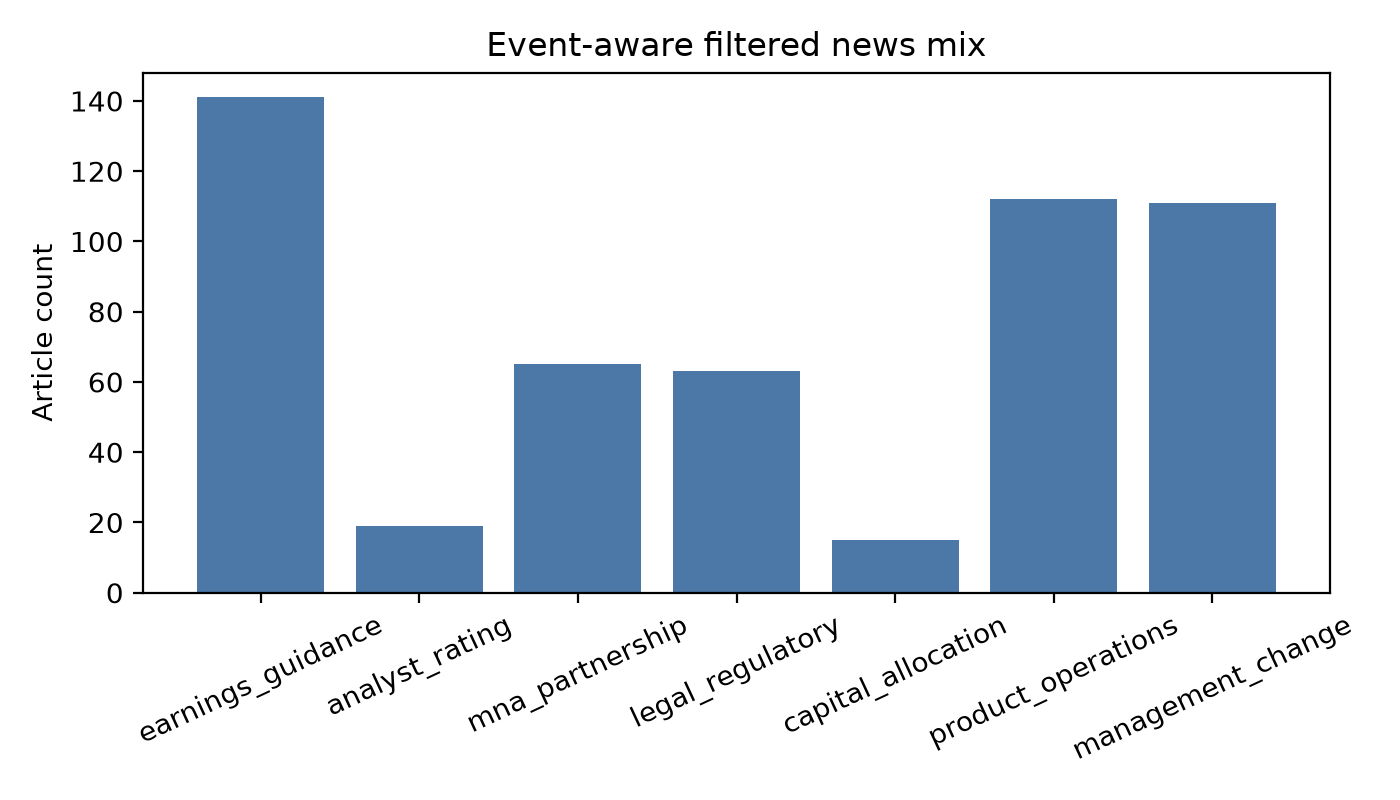
\includegraphics[width=\columnwidth]{figures/event_alpha_event_mix.png}
\caption{事件过滤后样本中的新闻类型分布}
\label{fig:eventmix}
\end{figure}

图\ref{fig:eventmix}显示，样本中最常见的事件为财报指引、产品运营和管理层变动，
其次是并购合作与法律监管。评级调整和资本配置数量较少，这说明公开新闻中真正具有
强交易解释性的事件并不均匀分布。

这种不均匀分布本身也是重要事实。若直接训练普通分类器，模型很容易被高频但低冲击
新闻主导；若先按经济含义进行事件过滤，模型至少能够区分“财报指引型情绪”和“产品
运营型情绪”。本文的规则taxonomy并不声称完整覆盖金融事件空间，而是提供一个低成本、
可复现、足以支撑课程论文实验的事件感知层。

\subsection{标签、基线与验证}

本文的目标不是下一日收盘方向，而是市场调整后的隔夜异常收益：
\begin{equation}
y^{ON}_{i,t+1} = \left(\frac{open_{i,t+1}}{close_{i,t}} - 1\right) - r^{MKT}_{t+1},
\end{equation}
其中$r^{MKT}_{t+1}$为SPY在同一隔夜窗口中的收益。该定义有两个好处：第一，它更接近
新闻在盘后到次日开盘之间被价格吸收的机制；第二，它剔除了市场整体夜间波动，使模型
更接近识别公司层面的alpha而不是beta。

基线特征为量价变量：1/5/20日收益、5日和20日波动率、5/20日均线差和成交量变化。
比较组则在其上加入事件感知情绪因子。模型采用Ridge和XGBoost回归，以覆盖线性与
非线性交互两类结构。验证方式包括：
\begin{itemize}[leftmargin=1.4em]
  \item \textbf{Static：}2019年训练，2020年测试；
  \item \textbf{Rolling：}过去6个月训练，下一个自然月测试。
\end{itemize}
评价指标则直接面向alpha识别：平均Pearson IC、平均rank IC、每天Top-Bottom异常
收益spread及其年化Sharpe。

其中IC衡量预测分数与真实异常收益之间的线性相关，rank IC衡量横截面排序的一致性。
由于真实交易中投资者通常不是买入所有预测为正的股票，而是按照信号强度进行排序，
rank IC比二分类准确率更适合评价alpha因子。Top-Bottom spread则进一步模拟每天做多
预测分数最高的股票、做空预测分数最低的股票所获得的异常收益差。由于本文样本股票数
仅为4只，spread应被解释为排序信号的原型验证，而不是完整投资组合回测。

\begin{equation}
IC_t = corr(\hat{y}_{i,t}, y^{ON}_{i,t}), \quad
RankIC_t = corr(rank(\hat{y}_{i,t}), rank(y^{ON}_{i,t})).
\end{equation}

\section{结果}

\subsection{事件感知情绪因子对非线性模型有正增量}

表\ref{tab:result}给出主要结果。Ridge在线性框架下并未从事件感知情绪中明显获益，
说明简单线性叠加不足以利用事件与价格之间的交互；而XGBoost在静态检验中，
\texttt{price+event}的rank IC由0.309提高到0.336，spread Sharpe由8.64提高到
9.11；在滚动重训中，rank IC由0.311提高到0.322，Sharpe由7.18提高到7.59。

\begin{table}[!htbp]
\centering
\caption{事件感知情绪因子结果}
\scriptsize
\setlength{\tabcolsep}{2.6pt}
\begin{tabular}{llcccc}
\toprule
模型 & 特征 & rank IC & Pearson IC & Spread & Sharpe\\
\midrule
Ridge & Price-static & .388 & .457 & .0164 & 9.29\\
Ridge & Price-rolling & .398 & .447 & .0171 & 9.29\\
Ridge & Event-static & .369 & .446 & .0160 & 9.03\\
Ridge & Event-rolling & .357 & .404 & .0157 & 8.47\\
XGB & Price-static & .309 & .392 & .0153 & 8.64\\
XGB & Price-rolling & .311 & .344 & .0138 & 7.18\\
XGB & Event-static & \textbf{.336} & \textbf{.403} & \textbf{.0161} & \textbf{9.11}\\
XGB & Event-rolling & \textbf{.322} & \textbf{.347} & \textbf{.0144} & \textbf{7.59}\\
\bottomrule
\end{tabular}
\label{tab:result}
\end{table}

\begin{figure}[!htbp]
\centering
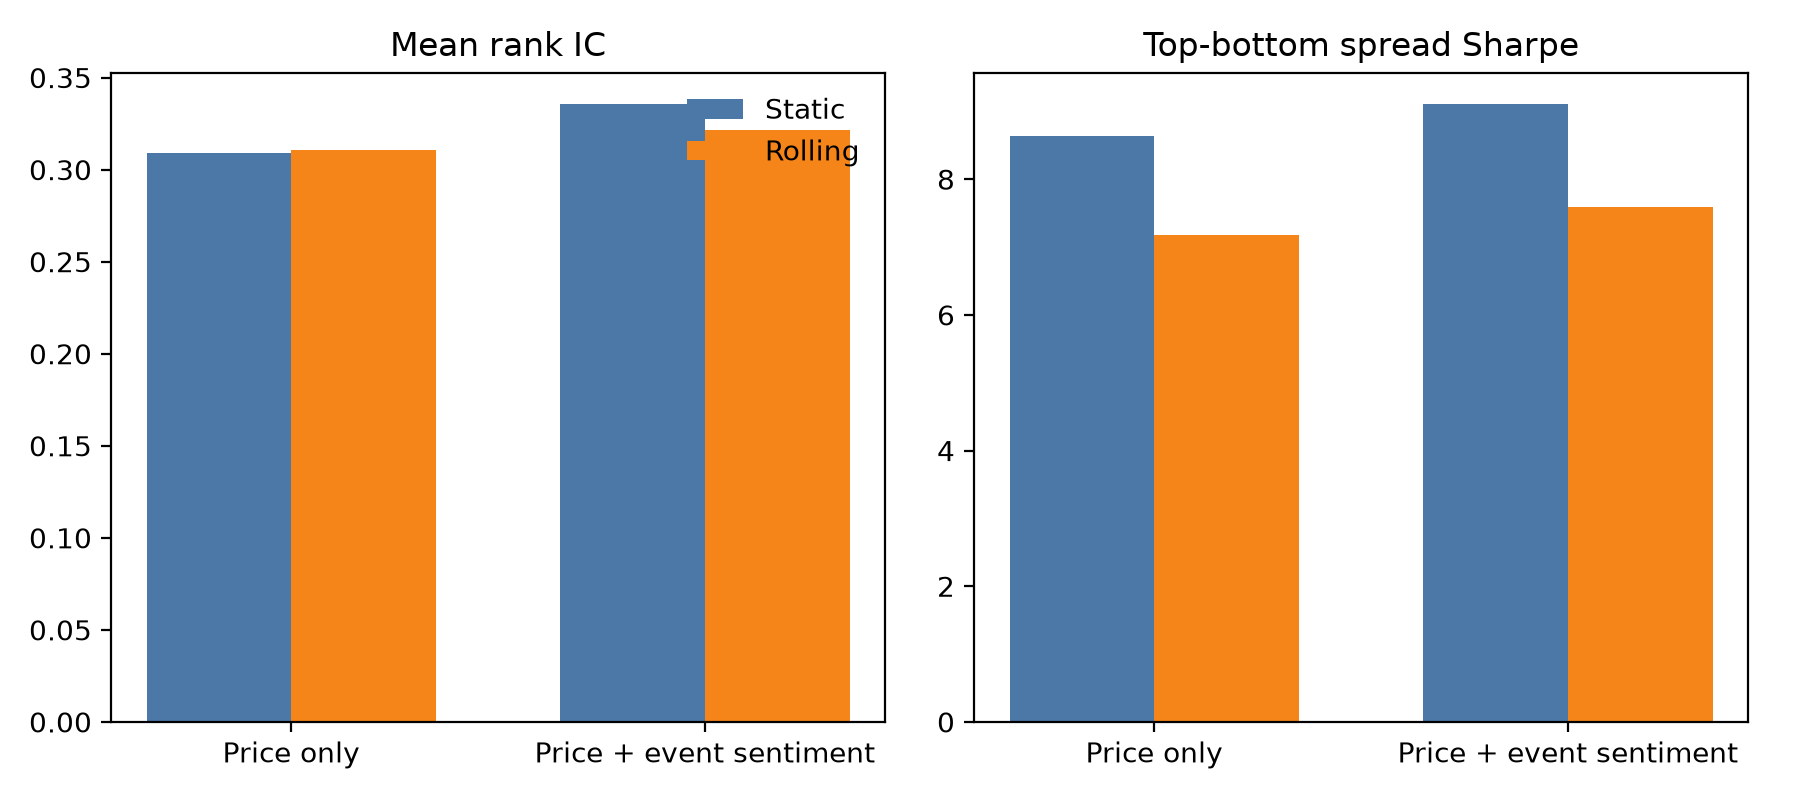
\includegraphics[width=\columnwidth]{figures/event_alpha_ic_comparison.png}
\caption{XGBoost下仅量价与事件感知情绪因子的rank IC与Sharpe比较}
\label{fig:ic}
\end{figure}

图\ref{fig:ic}表明，事件感知情绪因子的增量并不表现为“所有模型都变好”，而是更像
一种\textbf{非线性辅助因子}：只有当模型能够处理事件类别、情绪强度和价格状态之间的
交互时，事件情绪才更有机会转化为alpha。

这一点对解释结果很关键。Ridge模型加入事件因子后表现下降，说明事件标签和情绪强度
不是简单线性加总即可使用的变量。相同的事件在不同波动率、不同短期趋势和不同市场
状态下可能对应不同价格反应。例如，负面监管新闻在高波动阶段可能引发更强折价，而在
市场风险偏好较高时影响可能较弱。XGBoost的改进恰好说明，事件感知情绪更适合作为
与价格状态交互的条件变量，而不是独立的线性情绪因子。

\subsection{Top-Bottom spread具备持续正向累积}

图\ref{fig:spread}给出XGBoost Top-Bottom异常收益组合的累计净值。无论静态还是
滚动框架，加入事件感知情绪因子后的累计表现均高于仅量价基线，且静态框架下的提升
更明显。这说明该因子至少在当前样本上具备持续的横截面排序价值，而不是仅仅改善个别
极端日的回报。

需要强调的是，图\ref{fig:spread}中的累计净值不是完整实盘策略收益。它没有纳入真实
做空约束、融资成本、滑点、佣金和单股容量限制，也没有考虑新闻实际到达交易系统的
延迟。因此，该图的作用是检验排序信号是否具有持续方向，而不是证明该策略已经可以
直接上线。严格说，本文的证据支持“事件感知情绪因子具有原型alpha特征”，而不是支持
“已经形成生产级交易系统”。

\begin{figure}[!htbp]
\centering
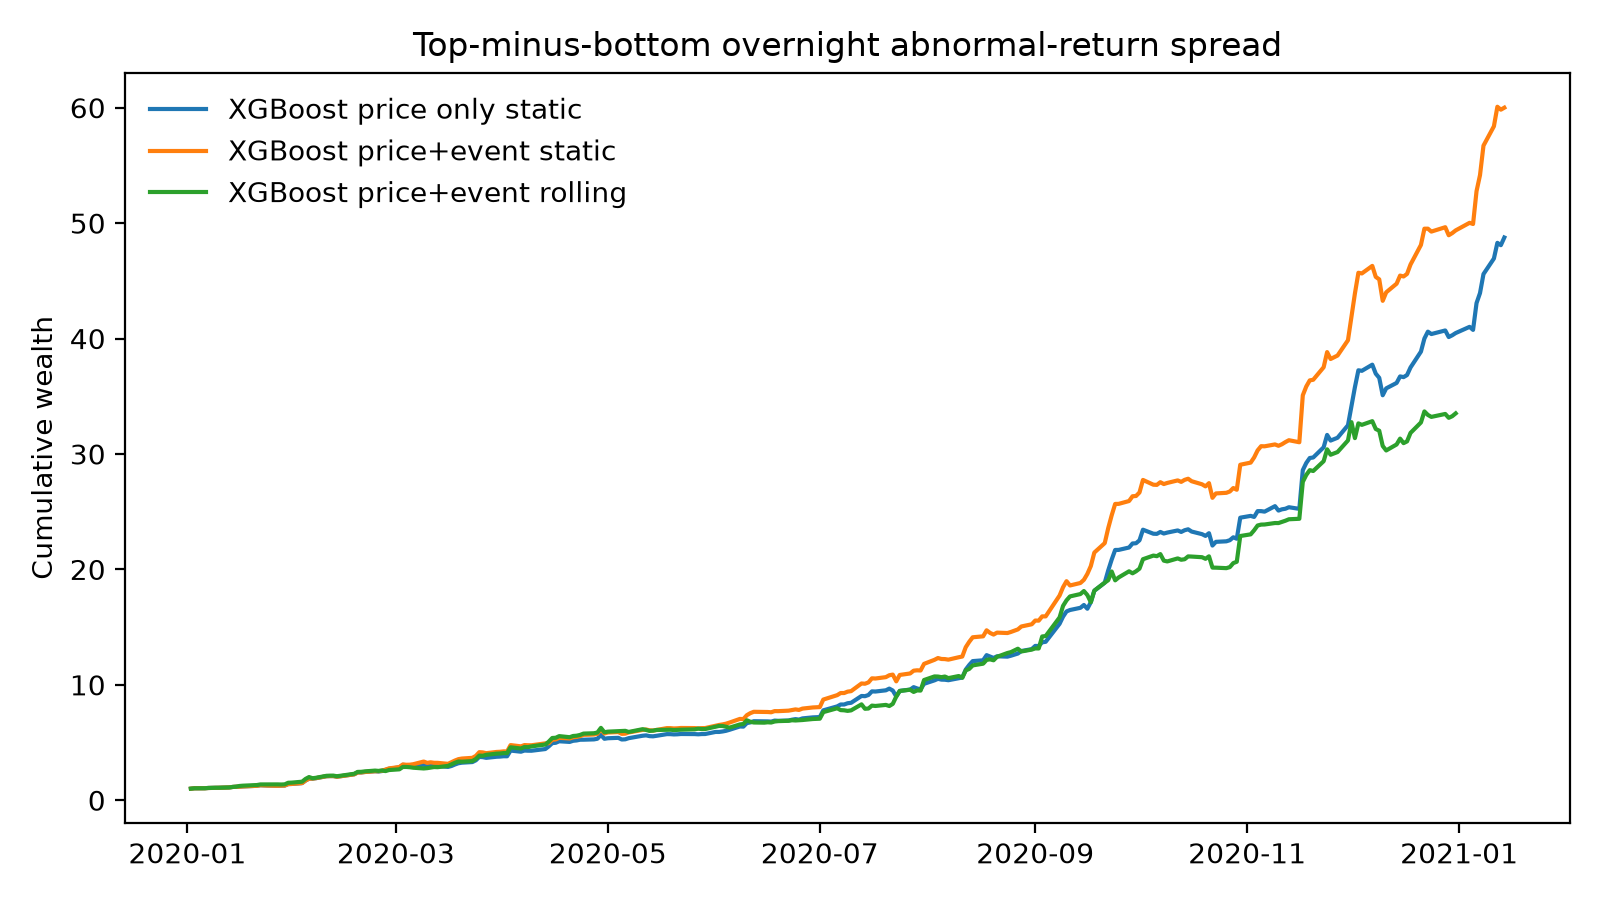
\includegraphics[width=\columnwidth]{figures/event_alpha_cumulative_spread.png}
\caption{XGBoost下Top-Bottom隔夜异常收益组合的累计净值}
\label{fig:spread}
\end{figure}

\subsection{可交易alpha来自“事件化情绪”，而不是平均情绪}

将结果与常见粗粒度情绪思路对比，可以得到一个更清楚的结论。本文并未证明“情绪分数
本身足够强”；相反，真正带来增量的是：先通过事件规则过滤掉低相关新闻，再把情绪绑定
到事件类型上，最后在更贴近新闻半衰期的隔夜窗口内评估。也就是说，alpha不是来自
平均语调，而是来自\textbf{事件语境中的情绪方向与强度}。

\section{讨论}

\subsection{为什么这个方向比“新闻情绪预测涨跌”更合理}

传统日级新闻情绪研究最大的问题，不是情绪完全无效，而是任务定义与交易机制错配。
一旦把目标改成公司级、事件过滤、隔夜异常收益，很多原本混在噪声里的信息会被重新
组织成更接近交易决策的因子。本文结果正说明了这一点：即使样本只有4只股票和两年，
事件感知情绪在XGBoost下仍然能稳定改善rank IC和spread Sharpe。

从论文写作角度看，这一结论比“情绪能预测涨跌”更严格。本文没有依赖全市场方向，也
没有把所有新闻混合成日度均值，而是先把可解释的事件筛出，再用异常收益和横截面排序
评价。这样得到的增量较小但更可信，因为它对应的是具体交易机制：在隔夜窗口中，公司
事件型新闻可能改变投资者对单只股票的相对定价。

\subsection{为什么我们仍然只把这看成第一版alpha原型}

本文仍有三点明显局限。第一，事件taxonomy是规则驱动的，无法覆盖更细的金融语义；
第二，样本只包含4只股票与2019--2020年窗口，足以验证框架，但不足以证明跨周期稳健性；
第三，午夜时间戳占比仍有16.47\%，说明公开新闻数据离真实毫秒级事件流还有距离。
因此，本文的最合理定位是：\textbf{在公开数据上把“事件感知情绪因子”这条alpha路线
跑通，而不是宣称已经得到可直接部署的生产级信号。}

此外，本文的结果存在一定样本选择风险。AAPL、GOOGL、MSFT和TSLA均属于高关注度、
高流动性股票，新闻传播速度快，市场反应也更充分。在小盘股或低关注股票中，新闻反应
可能更慢，事件感知情绪因子的半衰期可能更长；但在超大盘科技股中，信息也可能更快被
套利消化。因此，后续扩展到更宽股票池不仅是样本量问题，也是检验新闻alpha是否存在
横截面异质性的必要步骤。

\subsection{后续最有价值的升级方向}

若继续推进，最优先的不是换更复杂模型，而是三项数据与任务升级：第一，将当前规则
事件taxonomy升级为LLM或弱监督事件标注；第二，将数据底座从当前轻量新闻集迁移到
更大规模的FNSPID，以验证更近年份与更宽股票池；第三，把单一overnight窗口扩展为
1D、2D与3D多horizon，对比事件情绪alpha的半衰期。

\subsection{稳健性与评价边界}

本文采用静态划分和滚动重训两种验证方式，是为了避免单一年度划分造成偶然结论。静态
划分检验2019到2020的跨年迁移，滚动重训则更接近真实部署中“持续更新模型”的方式。
两种设置下XGBoost加入事件感知情绪均有正增量，说明结果不是单一划分下的孤立现象。
不过，本文没有进行多股票池、多年份和交易成本后的完整组合检验，因此仍应把结论限制
在“原型因子有效性”层面。严格的生产级验证还需要更长样本、更宽股票池和真实执行成本。

\section{结论}

本文直接回答的是“怎样做，才更有可能从金融新闻中识别可交易alpha”。我们的结论不是
继续使用日级平均情绪，而是：\textbf{必须把情绪细化为公司级、事件驱动、短窗口的因子。}
基于公开公司新闻数据，本文构造了事件感知情绪因子，并以市场调整后的隔夜异常收益
作为目标。在4只股票、2019--2020年的验证中，XGBoost模型加入事件感知情绪后，静态
rank IC从0.309提升到0.336，滚动rank IC从0.311提升到0.322，Top-Bottom spread
Sharpe也同步改善。研究表明，真正值得继续研究的不是粗粒度“新闻情绪预测股票涨跌”，
而是\textbf{事件感知情绪因子驱动的短期alpha识别}。

从研究意义上看，本文提供的不是一个最终答案，而是一个更合理的问题定义：若要研究
金融新闻情绪，就不应再停留于平均正负面分数，而应追问“哪类事件、指向哪家公司、在
哪个时间窗口、以何种情绪强度影响相对收益”。只有把这四个条件同时纳入，情绪研究才
更接近金融alpha研究，而不是普通文本分类任务。

\section{可复现性说明}

本文使用的脚本为 \texttt{code/event\_alpha\_experiment.py}，输入为
\texttt{data/2019\_processed.json.xz} 与 \texttt{data/2020\_processed.json.xz}，
输出保存在 \texttt{outputs/event\_alpha\_rerun/}。其中：
\begin{itemize}[leftmargin=1.4em]
  \item \texttt{metrics.csv} 保存表\ref{tab:result}对应指标；
  \item \texttt{diagnostics.json} 保存样本规模、时间分布和事件数量；
  \item \texttt{figures/event\_alpha\_event\_mix.png}、
  \texttt{event\_alpha\_ic\_comparison.png}、
  \texttt{event\_alpha\_cumulative\_spread.png}
  分别对应图\ref{fig:eventmix}、图\ref{fig:ic}和图\ref{fig:spread}。
\end{itemize}
主稿文件为 \texttt{paper\_rebuild\_xelatex.tex}，须用XeLaTeX编译。

\begin{thebibliography}{99}\scriptsize

\bibitem{tetlock}
Tetlock, P. C. Giving Content to Investor Sentiment: The Role of Media in the Stock Market.
\emph{The Journal of Finance}, 62(3):1139--1168, 2007.

\bibitem{lm}
Loughran, T., McDonald, B. When Is a Liability Not a Liability? Textual Analysis,
Dictionaries, and 10-Ks. \emph{The Journal of Finance}, 66(1):35--65, 2011.

\bibitem{tradetheevent}
Sawhney, R., Mathur, P., Mangal, R., Shah, R. Trade the Event: Corporate Events Detection
for News-Based Event-Driven Trading. \emph{Findings of ACL}, 2021.

\bibitem{efsa}
Li, Z., Liu, Y., Ren, X., et al. EFSA: Towards Event-Level Financial Sentiment Analysis.
\emph{ACL}, 2024.

\bibitem{targetsentiment}
Rizzo, T., et al. Benchmarking Large Language Models for Target-Based Financial Sentiment
Analysis. \emph{CLiC-it}, 2025.

\bibitem{eventawarefactor}
Wang, Y., et al. Event-Aware Sentiment Factors from LLM-Augmented Financial Tweets.
arXiv:2508.07408, 2025.

\bibitem{luckycat}
luckycat37. Financial News Dataset. Hugging Face Datasets, accessed on June 18, 2026.
\url{https://huggingface.co/datasets/luckycat37/financial-news-dataset}.

\end{thebibliography}

\end{document}
